\documentclass[12pt,handout]{beamer}
\usepackage[ngerman]{babel}
\usepackage[utf8]{inputenc}

% Thema
\usetheme{boxes}
% NOT \usecolortheme{fly}
\usefonttheme{structurebold}
%\useoutertheme{infolines}
\useoutertheme{infolines}

\beamertemplatenavigationsymbolsempty
%\setbeamertemplate{footline}[default]

% Weitere Pakete
\usepackage{amsmath,amsfonts,amssymb}
\usepackage{graphicx}
\usepackage{tabularx}
\usepackage{listings}
\usepackage{xcolor}

% Itemabstand vergrößern
\newlength{\wideitemsep}
\setlength{\wideitemsep}{\itemsep}
\addtolength{\wideitemsep}{1.5em}
\let\smallitem\item
\renewcommand{\item}{\setlength{\itemsep}{\wideitemsep}\smallitem}

\usepackage{textpos}
\setlength{\TPHorizModule}{1mm}
\setlength{\TPVertModule}{\TPHorizModule}

% C++
\def\CC{C\nolinebreak[4]\hspace{-.05em}\raisebox{.4ex}{\tiny\bf ++}\ }

% TODO Notiz
\newcommand\todo[1]{\textcolor{red}{TODO: #1}}

% Neue Befehle
\newcommand{\zB}{z.\,B.\ }
\newcommand{\dah}{d.\,h.\ }
\newcommand{\vgl}{vgl.\ }
\newcommand{\oae}{o.\,ä.\ }
\newcommand{\vlt}{vlt.\ }

% Listing
\lstset{ %
    language=C,                 % the language of the code
    basicstyle=\ttfamily,            % the size of the fonts that are used for the code
    breakatwhitespace=false,         % sets if automatic breaks should only happen at whitespace
    breaklines=true,                 % sets automatic line breaking
    stepnumber=2,                    % the step between two line-numbers. If it's 1, each line will be numbered
    tabsize=2,                       % sets default tabsize to 2 spaces
    morecomment=[l][\emph]{\#},
    captionpos=b,                    % sets the caption-position to bottom
}


\title[ERA GP Logikanalyzer]{Logikanalyzer\\\normalsize ERA Großpraktikum}
\author[]{Sven Hertle, Markus Engel, Thomas Czok}
\institute[]{Lehrstuhl für Rechnertechnik und Rechnerorganisation}
\date{22.07.2013}

\begin{document}
\begin{frame}{}
    \titlepage
\end{frame}

\begin{frame}{Gliederung}
    \tableofcontents
\end{frame}

\section{Was ist ein Logikanalyzer?}
\begin{frame}[<+->]{Was ist ein Logikanalyzer?}
    \begin{itemize}
        \item Messgerät für Zeitverlauf binärer Signale
        \item Ähnlich zum Oszilloskop, aber viele Eingänge und nur binäre Signale
        \item Debugging von digitalen Schaltungen
        \item Teilweise mehrere 100 Eingänge
    \end{itemize}
\end{frame}

\section{Funktionen und Features}
\begin{frame}[<+->]{Funktionen und Features}
    \begin{itemize}
        \item 8 Eingangskanäle
        \item VGA Ausgabe: 640x480 Pixel
        \item Steuerung über sieben Taster
        \item Aufnahme der Signale
            \begin{itemize}
                \smallitem Einmal Speicher voll schreiben (\todo{Anzahl Messwerte})
                \smallitem Speicher als Ring: Überschreiben alter Daten
            \end{itemize}
        \item Einstellbare Samplingrate: Maximum (\todo{ist was?}), 1ms, 10ms, 100ms, 1s
    \end{itemize}
\end{frame}
\begin{frame}[<+->]{Funktionen und Features}
    \begin{itemize}
        \item Scrollen in Aufnahme: Langsam und schnell
        \item Zoomen: 25\%, 50\%, 100\%, 200\%, 400\% \\
            100\% $\Leftrightarrow$ Ein Messwert pro Pixel
        \item Trigger pro Kanal: High, Low, Rising, Falling, Off \\
            Start, wenn alle Kriterien wahr sind
    \end{itemize}
\end{frame}

\section{Aufbau der Hardware}
\begin{frame}[<+->]{Aufbau der Hardware}
    \begin{figure}
        \centerline{
            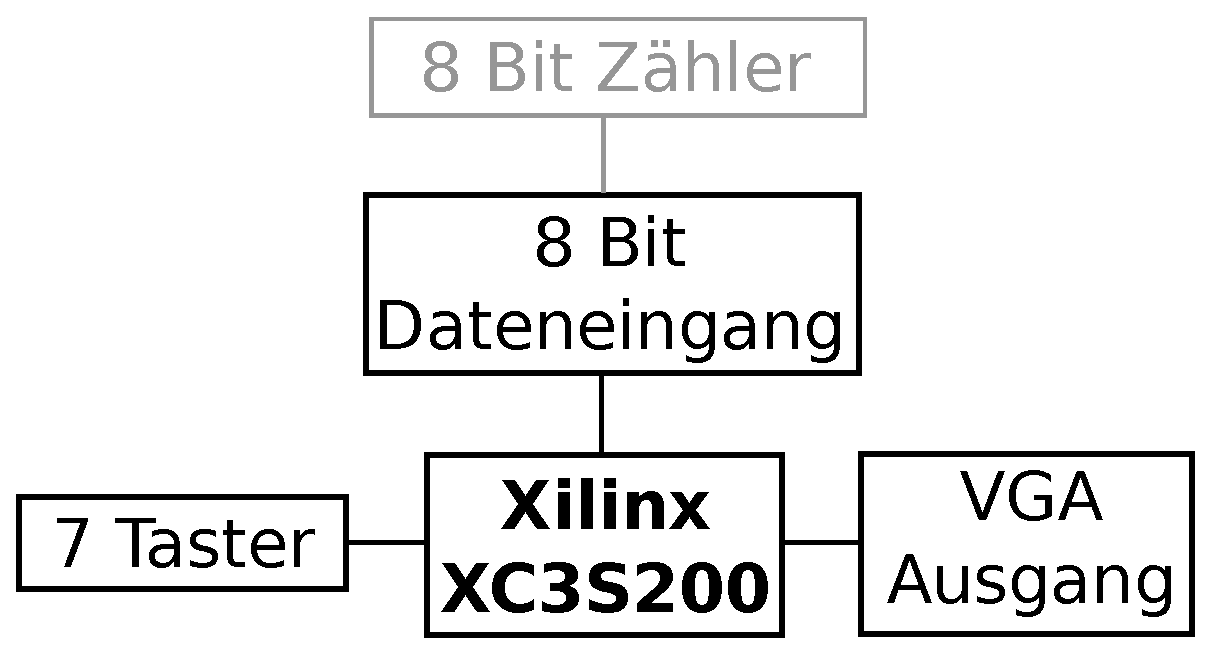
\includegraphics[width=0.8\textwidth]{abbildungen/hardware}
        }
    \end{figure}
\end{frame}

\section{Beschreibung der Komponenten}
\begin{frame}[<+->]{Beschreibung der Komponenten}
    \begin{figure}
        \centerline{
            \includegraphics[width=0.8\textwidth]{abbildungen/komponenten}
        }
    \end{figure}
\end{frame}
\begin{frame}[<+->]{Beschreibung der Komponenten}
    \begin{block}{Logikanalyzer}
        \begin{itemize}
            \item Steuerung der anderen Komponenten
            \item Speicherung der Signale mit Status des Logikanalyzers
            \item Auswerten der Taster und setzen der entsprechenden Signale
        \end{itemize}
    \end{block}
    \begin{block}{RAM}
        \begin{itemize}
            \item Dualport Block RAM
            \item Mit Core Generator erstellt
        \end{itemize}
    \end{block}
\end{frame}
\begin{frame}[<+->]{Beschreibung der Komponenten}
    \begin{block}{Sampler}
        \begin{itemize}
            \item Aufzeichnen der Messwerte im RAM
            \item Weitergabe der aktuellen Daten an Trigger
        \end{itemize}
    \end{block}
    \begin{block}{Sampler}
        \begin{itemize}
            \item Auswerten der aktuellen Messdaten
            \item Ausgabe eines Start Signals
        \end{itemize}
    \end{block}
\end{frame}
\begin{frame}[<+->]{Beschreibung der Komponenten}
    \begin{block}{VGA}
        \begin{itemize}
            \item Erzeugen des VGA Signals
            \item Eingabe: Alle Signale mit Statusinformationen
            \item Ergänzung von Flanken beim Zeichnen von Messwerten
        \end{itemize}
    \end{block}
    \begin{block}{VGA}
        \begin{itemize}
            \item Speicher für Schriftzeichen
            \item Schrift aus Linux Kernel mit 8x8 Pixel pro Zeichen
        \end{itemize}
    \end{block}
\end{frame}

\section{Projektverlauf und Probleme}
\begin{frame}[<+->]{Projektverlauf}
    \begin{itemize}
        \item Nutzung von GIT zur Versionskontrolle
        \item Erste Hälfte des Praktikums: VGA
        \item Danach: Implementierung des Logikanalyzers
    \end{itemize}
\end{frame}
\begin{frame}[<+->]{Probleme}
    \begin{itemize}
        \item Hardware: VGA anfangs falsch verbunden (HSYNC und VSYNC vertauscht)
        \item Erster Monitor unterstützte gewählte Auflösung und Frequenz nicht
        \item Zwei Teammitglieder abgesprungen
        \item Darstellung von Text verbraucht anfangs zu viel Platz
        \item Trigger: Steigende Flanken auf mehreren Kanälen nicht möglich
    \end{itemize}
\end{frame}


\setbeamercolor{background canvas}{bg=black}
\addtocounter{framenumber}{-1}
\frame[plain]{}

\end{document}
